\chapter{Hand Pose Recogntion using Deep Learning}
\begin{figure}[h!]
	\centering
	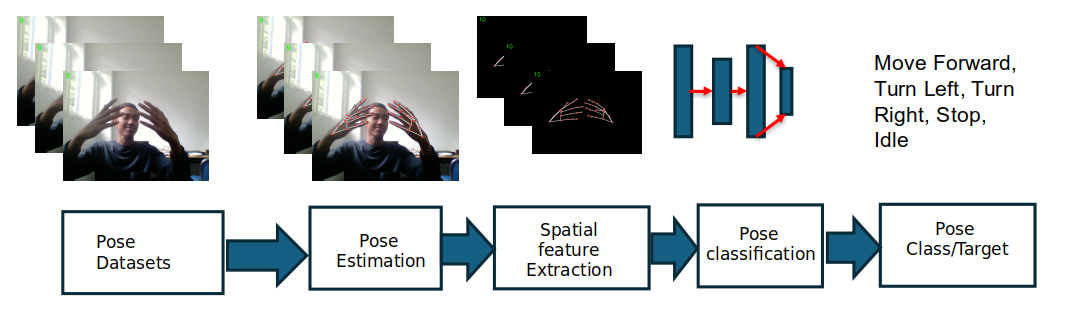
\includegraphics[width=\linewidth]{img/pose_pipeline} % Adjust the width or other parameters as needed
	\caption{Hand Recognition Pipeline}
	\label{fig:pose_pipeline} % Reference the figure in your text using \ref{fig:unique_label}
\end{figure}

\section{Dataset Acquisition}
This code provides a systematic way to acquire a dataset for hand pose recognition using Mediapipe and OpenCV. It captures hand landmarks and saves the corresponding frames from a webcam feed, enabling the creation of a labeled dataset for tasks like training gesture recognition models.

The process begins with the initialization and setup of necessary components. Mediapipe's Hands model is used for detecting and tracking hand landmarks, while OpenCV handles video capture and frame display. Command-line arguments allow customization of parameters such as the dataset path, label name, frame saving rate, maximum frames to save, and a delay before data collection starts. The script ensures that a directory for the dataset is created, organizing the captured data based on the provided label name.

Hand detection and landmark extraction are key steps in the process. The Mediapipe Hands model detects 21 landmarks on each hand, including knuckles and fingertips, and supports tracking up to two hands simultaneously. For every frame captured, the script converts it to RGB format and processes it using Mediapipe. Landmark coordinates are normalized relative to specific reference points, such as the wrist and a finger joint, making the data invariant to variations in hand size and position. The normalized landmarks for both hands are then concatenated into a single array, representing the frame’s hand pose data.

\section{Pose Estimation}

The `create\_dataset` function is a crucial part of the pose estimation process. It facilitates the acquisition of hand pose data by capturing frames from a webcam feed, extracting hand landmarks using Mediapipe's `Hands` solution, and organizing the data into labeled directories. This function serves as the foundation for building datasets tailored to pose estimation tasks, enabling further applications like gesture recognition and motion analysis.

Pose estimation involves detecting and interpreting key hand landmarks in real-time. The function initializes Mediapipe's `Hands` module, which is capable of identifying 21 specific landmarks on each hand, such as fingertips, joints, and the wrist. These landmarks represent the structural configuration of the hand and are essential for understanding its pose. By converting the captured video frames to RGB format and processing them through Mediapipe, the function extracts these landmarks with high precision.

To normalize the landmark data, the function computes positions relative to key reference points—namely, the wrist and a finger joint. This normalization step ensures that the data remains invariant to hand size and camera perspective, enhancing its generalizability for machine learning models. The landmark coordinates for both hands are flattened into a single array, representing the spatial configuration of the hands in each frame.

Beyond pose estimation, the `create\_dataset` function also incorporates real-time feedback and organization. Frames are captured and saved at user-defined intervals, allowing control over the frame rate and total number of frames collected. Each frame is stored in a labeled directory, organized by the name of the gesture or pose being recorded. The overlay of the detected landmarks on the video feed, along with a live counter of saved frames, enhances the usability of the function by providing visual confirmation and progress tracking.

This function exemplifies the integration of pose estimation techniques with practical data collection workflows. It not only extracts meaningful pose information but also structures the data in a format ready for subsequent analysis and model training. This makes it a powerful tool for researchers and developers working on applications in gesture recognition, human-computer interaction, and beyond.

\subsection{Import required Python libraries}
\begin{verbatim}
	import cv2
	import mediapipe as mp
	import numpy as np
	from datetime import datetime
	import os
	import time
	import argparse
\end{verbatim}

\subsection{MediaPipe Initialization}
\begin{lstlisting}
	mp_hands = mp.solutions.hands
	hands = mp_hands.Hands(static_image_mode=False,
	max_num_hands=2,
	min_detection_confidence=0.5,
	min_tracking_confidence=0.5)
	
\end{lstlisting}

This part initializes the Mediapipe Hands solution, which is responsible for detecting hand landmarks in video frames. The configuration allows real-time processing of up to two hands per frame, with parameters controlling the confidence thresholds for detection and tracking. This setup ensures accurate and stable landmark recognition during data collection.

\subsection{ Webcam Access and Directory Setup}

\begin{lstlisting}
cap = cv2.VideoCapture(0)
save_dir = os.path.join(direktori_path, nama_label)
if not os.path.exists(save_dir):
	os.makedirs(save_dir)
	
\end{lstlisting}

The webcam is opened using OpenCV’s VideoCapture, which serves as the data source for real-time frame capture. The save\_dir is created dynamically based on the dataset path and label name, ensuring an organized directory structure for storing the collected data.

\subsection{Landmark Extraction}
\begin{lstlisting}
def ekstraksi_fitur(frame):
frame_rgb = cv2.cvtColor(frame, cv2.COLOR_BGR2RGB)
results = hands.process(frame_rgb)
height, width, _ = frame.shape
...
# Normalization and concatenation of landmarks
return np.concatenate((left_hand_landmarks.flatten(), right_hand_landmarks.flatten()))

\end{lstlisting}

This function extracts and processes hand landmarks from each frame:
\begin{enumerate}
	\item Conversion to RGB: Mediapipe requires frames in RGB format for processing.
	\item Landmark Processing: If hand landmarks are detected, their coordinates are normalized relative to reference points (e.g., the wrist and a finger joint) to ensure invariance to hand size and position.
	\item Concatenation: The landmarks for both hands are flattened and concatenated into a single array, representing the full pose information for the frame.
\end{enumerate}


\section{Geometric Feature Extraction}
\section{Model Architecture}

\section{Pose Classification}
\section{Pose Inference}